\documentclass[11pt,a4paper]{report}
\usepackage{exscale,times}
\usepackage{graphicx}
\usepackage{epstopdf}
\usepackage{amsmath,amsthm,amssymb}
\usepackage{epsfig}
\usepackage{latexsym}
\usepackage{amssymb}
\usepackage{german}
\setlength{\parindent}{0pt}
\setlength{\parskip}{5pt plus 2pt minus 1 pt}
\topmargin  -5mm
\evensidemargin 8mm
\oddsidemargin  2mm
\textwidth  158mm
\textheight 230mm
\frenchspacing
\sloppy
\newcommand{\xvec}{\bold{x}}
\newcommand{\vvec}{\bold{v}}
\newcommand{\wvec}{\bold{w}}
\newcommand{\evec}{\bold{e}}
\newcommand{\nuvec}{\bold{\nu}}
\newcommand{\R}[1]{\mathbb{R}^{#1}}
\newcommand{\setR}{\mathbb{R}}
\newcommand{\p}{$p$}
\newcommand{\norm}[2][2]{\|#2 \|_#1}
\newcommand{\diver}{\text{div}}
\newcommand{\refer}[1]{(\ref{#1})}
\newcommand{\ndof}{\text{ndof}}
\newcommand{\gauss}[2]{e^{-\frac{(\vvec #2)^2}{#1}}}
\newcommand{\lagrange}[2]{l_i(\frac{\vvec #2}{\sqrt{#1}})}


\begin{document}
\begin{center}
\textbf{10. \"Ubung Numerik von partiellen Differentialgleichungen - station\"are Probleme} \newline 
\textbf{13. J\"anner 2022}
\end{center}

\setcounter{enumi}{4}

\begin{enumerate}

\item {\em Minimierungsproblem mit Nebenbedingungen}. Betrachten Sie
  $$
  \min_{v \in V \atop b(v,q) = g(q) \forall \,q \in Q}  J(v)
  $$
  mit dem Funktional 
  $$
  J(v) = \tfrac{1}{2} \,  a(v,v) - f(v)
  $$
 mit $a(.,.)$ symmetrisch und elliptisch,  $b(.,.)$ erf\"ulle die LBB
 - Bedingung, und alle Formen stetig auf den Hilbertr\"aumen $V$
 bzw. $Q$.

 Zeigen Sie dass das Minimierungsproblem mit Nebenbedingungen
 eindeutig l\"osbar ist. Starten Sie mit homogenen Nebenbedingungen
 (d.h. $g(.)=0$), und f\"uhren Sie den allgemeinen Fall darauf
 zur\"uck (vgl: Homogensierung von Dirichlet Randbedingungen).

\item {\em Lagrangefunktion.} Geben Sie die dazugeh\"orige
 Lagrangefunktion 
 $$
 L(u,p) = ??
 $$
an. Bestimmen Sie Gleichungen f\"ur das Vorliegen von kritischen
Punkten von der Lagrangefunktion (Richtungsableitungen nach $v$ bzw
$q$ m\"ussen 0 sein). Verwenden Sie einen passenden Satz um die
Existenz einer eindeutigen L\"osung $(u,p) \in V \times Q$ zu erhalten.

Zeigen Sie dass $L(.,.)$ im ersten Argument srikt konvex ist, und im
zweiten Argument (nicht strikt) konkav ist, und 
$$
L(v,p) \geq L(u,p) \geq L(u,q) \qquad \forall \, v \in V, \; \forall
\, q \in Q,
$$
d.h. der kritische Punkt $(u,p)$ ist ein Sattelpunkt.

Definieren Sie weiters die duale Funktion
$$
J^\ast(q) := \inf_{v \in V} L(v,q)
$$
und zeigen Sie dass
$$
\sup_{q \in Q} J^\ast (q)
$$
ebenfalls eindeutig l\"osbar ist mit der gleichen L\"osung $p$.
Hierzu ist es geschickt mit Operatoren $A$ und $B$ zu arbeiten.

\item Implementieren Sie einen FEM-Raum mit Raviart-Thomas Elementen
  niedrigster Ordnung.

  Teilaufgaben:
  \begin{itemize}
  \item Rechnen Sie am Referenzdreieck nach dass die Basisfunktion
    zur Kante $[V_i, V_j]$ 
  $$
  \lambda_i \nabla^\bot \lambda_j - \lambda_j \nabla^\bot \lambda_i
  $$
  ist, wobei $\nabla^\bot := (\partial_y, -\partial_x)$ der um 90 Grad
  gedrehte Gradient ist.
  \item Folgen Sie der Implementierung der $H^1$ - Elemente
    \item Jetzt sind die Basisfunktionen Vektor-wertig, der
      nat\"urliche Differentialoperator $\operatorname{div}$ hingegen
      Skalar-wertig.
    \item Die Abbildung vom Referenzelement auf das physikalische
      passiert mit der Piola - Transformation, die geht in die beiden {\tt
        DiffOp} Klassen ein.
    \item Verwenden Sie zur konsistenten Orientierung der Kanten die
      globalen Vertexnummern, Vorlage {\tt HighOrderFiniteElement}.
    \end{itemize}

  \item {\it Prager-Synge}. Betrachten die das Variationsproblem: Ges
    $u \in H^1, u = u_D$ on $\Gamma_D$ sodass
    $$
    \int \lambda \nabla u \nabla v = \int f v + \int_{\Gamma_N} g v \qquad \forall \, v \in
    H^1, v = 0 \text{ on } \Gamma_D.
    $$
    Sei nun $v_h$ sodass $v_h = u_D$, und $\tau_h \in \Sigma_h
    \subset H(\operatorname{div})$ mit $\operatorname{div} \tau_h = -f$ und $\tau_h
    \cdot n = -g$ auf $\Gamma_N$. Diese $v_h$ und $\tau_h$ sind typischerweise
    FEM - L\"osungen $u_h$ und $\sigma_h$ der primalen bzw. der
    gemischten Variationsformulierung, m\"ussen aber nicht.

    Zeigen Sie:
    \begin{itemize}
      \item Orthogonalit\"at der Fehler:
        $$
        \int_\Omega  \nabla (u - v_h) (\lambda \nabla u - \tau_h) = 0
        $$
      \item Pythagoras:
        $$
        \|  \nabla v_h  - \lambda^{-1} \sigma_h  \|_\lambda^2 =
        \| \nabla u - \nabla v_h \|_\lambda^2 +
        \| \nabla u - \lambda^{-1} \sigma_h  \|_\lambda^2 
        $$
        mit der Norm $\| \cdot \|_\lambda := \big( \int \lambda |
        \cdot |^2
        \big) ^{1/2}$.

      \item Thales-Kreis:
        Wir setzen
        $$
        \sigma_h^\ast = \tfrac{1}{2} \big( \lambda \nabla v_h + \tau_h \big)
        $$
        Dann gilt:
        $$
        \| \nabla u - \lambda^{-1} \sigma_h^\ast \|_\lambda = \tfrac{1}{2} \|
        \nabla v_h - \lambda^{-1} \tau_h \|_\lambda
        $$
      \end{itemize}

    \begin{center}
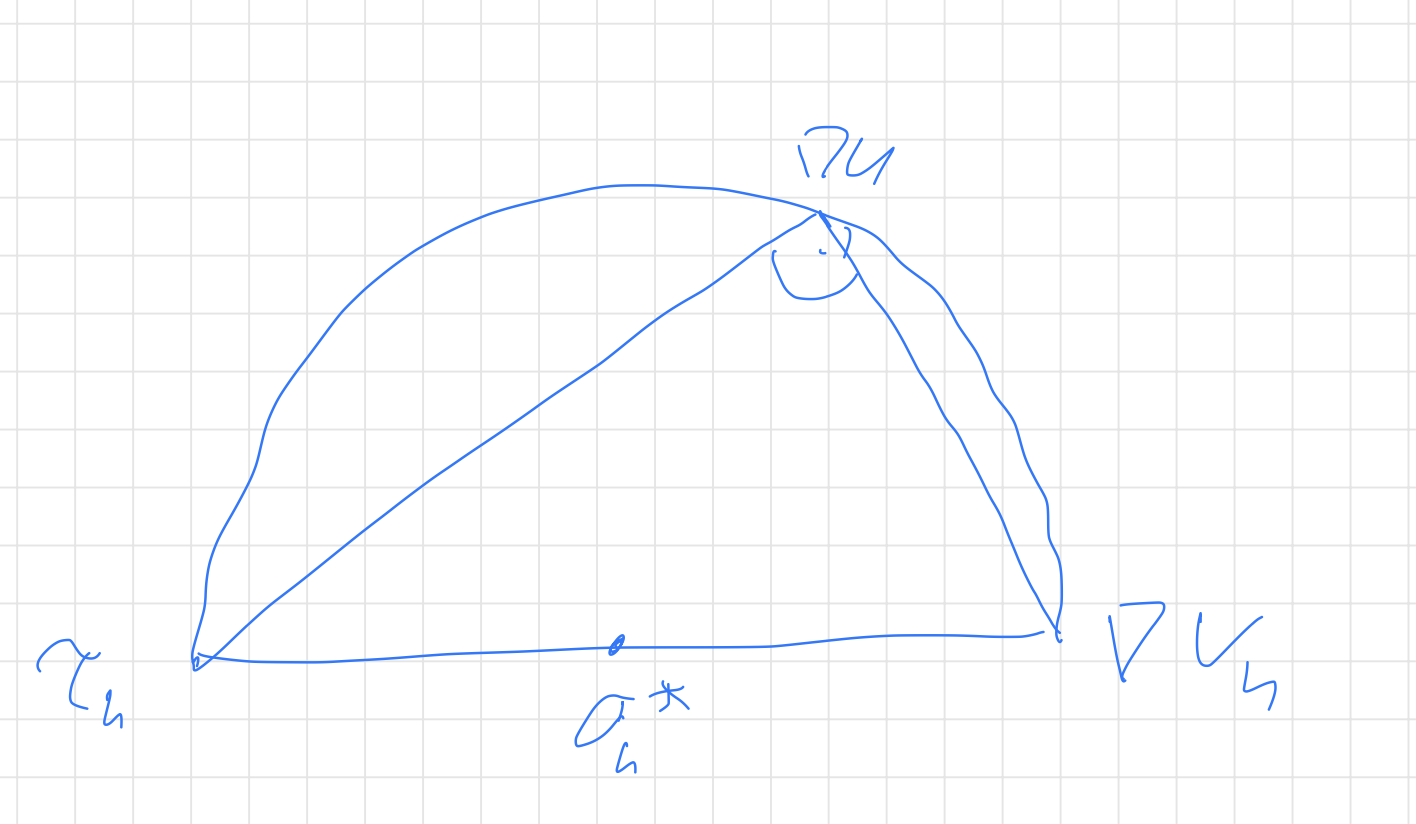
\includegraphics[width=0.3\textwidth]{Thales.png}
\end{center}
      
Bestimmen Sie $u_h$, $\sigma_h$ und $\sigma_h^\ast$ (f\"ur unser Bsp
aus \"U2.1) numerisch, und
berechnen Sie den Fehler von $\sigma_h^\ast$.
      
\end{enumerate}

\bigskip

\centerline{Frohe Weihnachten und Alles Gute f\"ur 2022}
\end{document}